\documentclass[12pt,a4paper]{article}

% ─── Page Layout ───────────────────────────────────────────────────────────────
\usepackage[a4paper, margin=0.8in, headheight=14pt]{geometry}

% ─── Fonts (XeLaTeX) ───────────────────────────────────────────────────────────
\usepackage{fontspec}
\usepackage{unicode-math}
\setmainfont{TeX Gyre Pagella}
\setmonofont[Scale=0.88]{TeX Gyre Cursor}
\setmathfont{Latin Modern Math}

% ─── Packages ──────────────────────────────────────────────────────────────────
\usepackage{xcolor}
\usepackage{colortbl}
\usepackage{titlesec}
\usepackage{enumitem}
\usepackage{tabularx}
\usepackage{booktabs}
\usepackage{array}
\usepackage{amsmath}
\usepackage{tikz}
\usetikzlibrary{shapes.geometric, arrows.meta, positioning, calc, fit, decorations.pathreplacing}
\usepackage{tcolorbox}
\tcbuselibrary{skins, breakable}
\usepackage{hyperref}
\usepackage{fancyhdr}
\usepackage{graphicx}
\usepackage{microtype}
\usepackage{caption}
\usepackage{setspace}
\usepackage{multirow}
\usepackage{tocloft}

% ─── Q&A helper ────────────────────────────────────────────────────────────────
\newcommand{\Q}[1]{\textbf{#1}\par\noindent\ignorespaces}

% ─── Colour Palette ────────────────────────────────────────────────────────────
\definecolor{myred}{RGB}{196,30,58}
\definecolor{mydark}{RGB}{30,30,50}
\definecolor{mygreen}{RGB}{14,120,80}
\definecolor{myteal}{RGB}{0,130,140}
\definecolor{myamber}{RGB}{180,100,0}
\definecolor{mypurple}{RGB}{100,30,160}
\definecolor{mygray}{RGB}{246,247,249}
\definecolor{mgframe}{RGB}{180,185,200}
\definecolor{watermark}{RGB}{195,200,215}
\definecolor{hdrred}{RGB}{250,232,235}
\definecolor{hdrgreen}{RGB}{220,244,233}
\definecolor{hdrteal}{RGB}{220,242,244}
\definecolor{hdramber}{RGB}{253,242,215}
\definecolor{hdrpurple}{RGB}{238,228,255}
\definecolor{hdrgray}{RGB}{238,240,245}
\definecolor{rowalt}{RGB}{250,251,253}

% ─── Section Formatting ────────────────────────────────────────────────────────
\titleformat{\section}
  {\large\bfseries\color{myred}}{\thesection.}{0.5em}{}
  [\vspace{1pt}{\color{myred}\rule{\linewidth}{0.8pt}}]
\titleformat{\subsection}
  {\normalsize\bfseries\color{mydark}}{\thesubsection}{0.5em}{}
\titlespacing*{\section}{0pt}{18pt}{7pt}
\titlespacing*{\subsection}{0pt}{11pt}{4pt}

% ─── Paragraph ─────────────────────────────────────────────────────────────────
\setlength{\parindent}{0pt}
\setlength{\parskip}{4pt}

% ─── TOC Styling ───────────────────────────────────────────────────────────────
\renewcommand{\cfttoctitlefont}{\large\bfseries\color{myred}}
\renewcommand{\cftaftertoctitle}{\par\noindent{\color{myred}\rule{\linewidth}{0.8pt}}}
\setlength{\cftbeforetoctitleskip}{0pt}
\setlength{\cftaftertoctitleskip}{6pt}
\renewcommand{\cftsecfont}{\normalsize\bfseries\color{mydark}}
\renewcommand{\cftsecpagefont}{\normalsize\bfseries\color{myteal}}
\renewcommand{\cftsecleader}{\cftdotfill{\cftdotsep}}
\setlength{\cftbeforesecskip}{7pt}
\renewcommand{\cftsubsecfont}{\small\color{mydark}}
\renewcommand{\cftsubsecpagefont}{\small\color{myteal}}
\setlength{\cftbeforesubsecskip}{3pt}
\setlength{\cftsubsecindent}{1.4em}

% ─── Table helpers ─────────────────────────────────────────────────────────────
\renewcommand{\arraystretch}{1.45}
\setlength{\tabcolsep}{6pt}
\newcolumntype{B}[1]{>{\small\bfseries\raggedright\arraybackslash}p{#1}}
\newcolumntype{Y}{>{\small\raggedright\arraybackslash}X}

% ─── Header / Footer ───────────────────────────────────────────────────────────
\pagestyle{fancy}
\fancyhf{}
\fancyhead[L]{\small\color{myred}\textbf{EC602}\;\color{mydark}--- Computer Network}
\fancyhead[R]{\small\color{myteal}\textbf{Module 1 Notes}}
\fancyfoot[C]{\small\color{mydark}\thepage}
\fancyfoot[R]{\small\color{watermark}\textit{© Biraj}}
\renewcommand{\headrulewidth}{0.5pt}
\renewcommand{\footrulewidth}{0.3pt}

% ─── Hyperref ──────────────────────────────────────────────────────────────────
\hypersetup{
  colorlinks=true, linkcolor=myteal, urlcolor=myteal,
  pdfauthor={Biraj Sarkar},
  pdftitle={EC602 --- Module 1 Notes}
}

% ─── tcolorbox styles ──────────────────────────────────────────────────────────
\tcbset{
  tikzbox/.style={
    colback=mygray, colframe=mgframe, boxrule=0.6pt, arc=4pt,
    left=8pt, right=8pt, top=6pt, bottom=6pt,
    colbacktitle=mgframe, coltitle=mydark,
    fonttitle=\small\bfseries
  },
  defbox/.style={
    colback=hdrgreen, colframe=mygreen, boxrule=0.8pt, arc=4pt,
    left=9pt, right=9pt, top=6pt, bottom=6pt,
    colbacktitle=mygreen, coltitle=white,
    fonttitle=\small\bfseries
  },
  formulabox/.style={
    colback=hdrteal, colframe=myteal, boxrule=0.8pt, arc=4pt,
    left=9pt, right=9pt, top=7pt, bottom=7pt,
    colbacktitle=myteal, coltitle=white,
    fonttitle=\small\bfseries
  },
  examplebox/.style={
    colback=hdramber, colframe=myamber, boxrule=0.8pt, arc=4pt,
    left=9pt, right=9pt, top=6pt, bottom=6pt,
    colbacktitle=myamber, coltitle=white,
    fonttitle=\small\bfseries
  },
  masonbox/.style={
    colback=hdrpurple, colframe=mypurple, boxrule=0.8pt, arc=4pt,
    left=9pt, right=9pt, top=6pt, bottom=6pt,
    colbacktitle=mypurple, coltitle=white,
    fonttitle=\small\bfseries
  },
  exambox/.style={
    colback=hdrpurple, colframe=mypurple, boxrule=1pt, arc=5pt,
    left=10pt, right=10pt, top=8pt, bottom=8pt,
    colbacktitle=mypurple, coltitle=white,
    fonttitle=\bfseries,
    breakable
  }
}
% Make all boxes breakable across pages
\tcbset{breakable}

% ─── TikZ styles ───────────────────────────────────────────────────────────────
\tikzset{
  block/.style={rectangle, draw=myteal, fill=hdrteal,
    text width=2.4cm, align=center, minimum height=0.95cm,
    font=\small, rounded corners=3pt, line width=0.7pt},
  redblock/.style={rectangle, draw=myred, fill=hdrred,
    text width=2.4cm, align=center, minimum height=0.95cm,
    font=\small, rounded corners=3pt, line width=0.7pt},
  netnode/.style={rectangle, draw=myteal, fill=hdrteal,
    text width=1.5cm, align=center, minimum height=0.8cm,
    font=\small, rounded corners=3pt, line width=0.7pt},
  arrow/.style={-Stealth, thick, color=mydark},
  redarrow/.style={-Stealth, thick, color=myred},
  line/.style={thick, color=mydark}
}

% ═══════════════════════════════════════════════════════════════════════════════
\begin{document}
% ═══════════════════════════════════════════════════════════════════════════════

\begin{center}
  {\LARGE\bfseries\color{myred} EC602 --- Computer Network}\\[5pt]
  {\normalsize\color{mydark} Semester VI \quad$\bullet$\quad 3L:0T:0P \quad$\bullet$\quad 3 Credits}\\[3pt]
  {\normalsize\color{myteal}\textbf{Module 1 Exam Notes}}\\[3pt]
  {\small\color{mydark} CGEC \;$|$\; B.Tech ECE (2023--27) \;$|$\; \textit{Biraj Sarkar}}
\end{center}
\vspace{2pt}
\noindent{\color{myred}\rule{\linewidth}{1.5pt}}
\vspace{2pt}

\tableofcontents
\newpage

%═══════════════════════════════════════════════════════════════════════════════
\section{Overview of Data Communication and Networking}
%═══════════════════════════════════════════════════════════════════════════════

\begin{tcolorbox}[defbox]
\textbf{Data Communication:} The exchange of data between two devices via a transmission medium. It requires a \textit{sender}, \textit{receiver}, \textit{message}, \textit{medium}, and \textit{protocol}.
\end{tcolorbox}

\subsection{Components of Data Communication}

\begin{tabularx}{\linewidth}{|B{3.2cm}|X|}
\hline
\rowcolor{hdrgreen}
\multicolumn{1}{|>{\centering\arraybackslash}p{3.2cm}|}{\textbf{\color{mygreen}Component}} &
\multicolumn{1}{>{\centering\arraybackslash}X|}{\textbf{\color{mygreen}Description}} \\
\hline
Message        & The information (data) to be communicated --- text, numbers, images, audio, video. \\
\hline
\rowcolor{rowalt}
Sender         & The device that sends the data message (computer, phone, camera). \\
\hline
Receiver       & The device that receives the message (computer, printer, phone). \\
\hline
\rowcolor{rowalt}
Medium         & The physical path over which the message travels (cable, air, fibre). \\
\hline
Protocol       & A set of rules governing data communication; ensures sender and receiver agree on format, timing, and error handling. \\
\hline
\end{tabularx}

\subsection{Data Representation}

Data is represented in different formats depending on the type of information:\par\noindent
\begin{tabularx}{\linewidth}{|B{3.0cm}|X|}
\hline
\rowcolor{hdrteal}
\multicolumn{1}{|>{\centering\arraybackslash}p{3.0cm}|}{\textbf{\color{myteal}Type}} &
\multicolumn{1}{>{\centering\arraybackslash}X|}{\textbf{\color{myteal}Representation}} \\
\hline
Text           & Encoded using bit patterns --- \textbf{ASCII} (7-bit, 128 chars), \textbf{ISO 8859} (8-bit, 256 chars), \textbf{Unicode} (32-bit, universal). \\
\hline
\rowcolor{rowalt}
Numbers        & Stored directly in binary; not converted to ASCII to save space. \\
\hline
Images         & Represented as a matrix of pixels; each pixel encoded in bits (RGB). \\
\hline
\rowcolor{rowalt}
Audio          & Continuous signal sampled at regular intervals and quantised to binary values. \\
\hline
Video          & Sequence of images (frames) displayed at a rate (fps) to create motion. \\
\hline
\end{tabularx}

\subsection{Direction of Data Flow}

\begin{tcolorbox}[tikzbox, title={Data Flow Modes}]
\centering
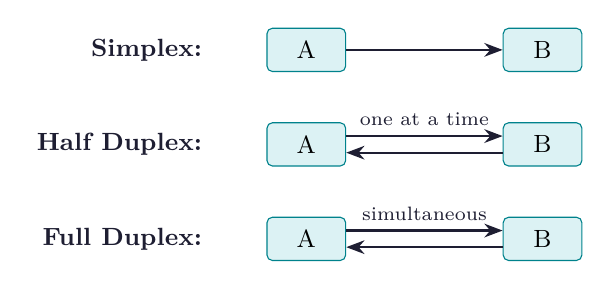
\begin{tikzpicture}[
  dev/.style={rectangle, draw=myteal, fill=hdrteal, minimum width=1.0cm, minimum height=0.55cm, align=center, font=\small, rounded corners=2pt},
  lbl/.style={font=\small\bfseries\color{mydark}, anchor=east}
]
% Simplex
\node[lbl] at (0, 3.0) {Simplex:};
\node[dev] (SA) at (1.2, 3.0) {A};
\node[dev] (SB) at (4.2, 3.0) {B};
\draw[arrow] (SA) -- (SB);

% Half Duplex
\node[lbl] at (0, 1.8) {Half Duplex:};
\node[dev] (HA) at (1.2, 1.8) {A};
\node[dev] (HB) at (4.2, 1.8) {B};
\draw[arrow] ([yshift=3pt]HA.east) -- node[above, font=\scriptsize] {one at a time} ([yshift=3pt]HB.west);
\draw[arrow] ([yshift=-3pt]HB.west) -- ([yshift=-3pt]HA.east);

% Full Duplex
\node[lbl] at (0, 0.6) {Full Duplex:};
\node[dev] (FA) at (1.2, 0.6) {A};
\node[dev] (FB) at (4.2, 0.6) {B};
\draw[arrow] ([yshift=3pt]FA.east) -- node[above, font=\scriptsize] {simultaneous} ([yshift=3pt]FB.west);
\draw[arrow] ([yshift=-3pt]FB.west) -- ([yshift=-3pt]FA.east);
\end{tikzpicture}
\end{tcolorbox}

\begin{tabularx}{\linewidth}{|B{3.0cm}|X|X|}
\hline
\rowcolor{hdrgray}
\multicolumn{1}{|>{\centering\arraybackslash}p{3.0cm}|}{\textbf{Mode}} &
\multicolumn{1}{>{\centering\arraybackslash}X|}{\textbf{Description}} &
\multicolumn{1}{>{\centering\arraybackslash}X|}{\textbf{Example}} \\
\hline
Simplex        & One direction only; receiver cannot send back. & TV broadcast, keyboard to CPU \\
\hline
\rowcolor{rowalt}
Half Duplex    & Both directions, but \textbf{not simultaneously}; one at a time. & Walkie-talkie, CB radio \\
\hline
Full Duplex    & Both directions \textbf{simultaneously}; uses two separate channels or frequencies. & Telephone, mobile call \\
\hline
\end{tabularx}

\subsection{Network Criteria}

A good network must satisfy three fundamental criteria:

\begin{tcolorbox}[formulabox, title={\textbf{Three Criteria of a Good Network}}]
\begin{enumerate}[label=\textbf{\arabic*.}, leftmargin=*, itemsep=4pt, topsep=0pt]
  \item \textbf{Performance} --- measured by transit time (time for a message to travel from sender to receiver) and response time. Affected by number of users, type of medium, hardware, and software.
  \item \textbf{Reliability} --- frequency of failure, recovery time after failure, robustness in catastrophe.
  \item \textbf{Security} --- protecting data from unauthorised access, damage, and implementing recovery policies.
\end{enumerate}
\end{tcolorbox}

%═══════════════════════════════════════════════════════════════════════════════
\section{Physical Structure: Topology and Categories}
%═══════════════════════════════════════════════════════════════════════════════

\subsection{Network Topologies}

\begin{tcolorbox}[defbox]
\textbf{Topology:} The geometric arrangement of devices (nodes) and links in a network. It defines how devices are physically or logically connected.
\end{tcolorbox}

\begin{tcolorbox}[tikzbox, title={Common Network Topologies}]
\centering
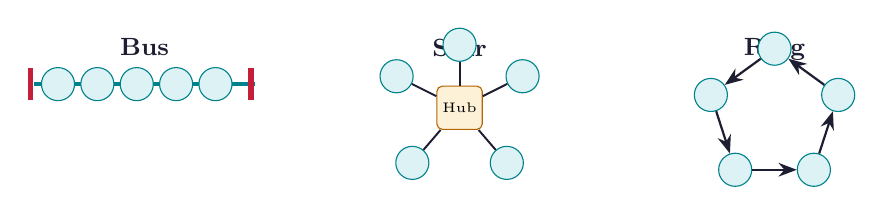
\begin{tikzpicture}[
  dev/.style={circle, draw=myteal, fill=hdrteal, minimum size=0.42cm, inner sep=0pt},
  hub/.style={rectangle, draw=myamber, fill=hdramber, minimum size=0.55cm, inner sep=2pt, font=\tiny, rounded corners=2pt},
  lbl/.style={font=\small\bfseries\color{mydark}, anchor=north}
]

%--- BUS (left) ---
\node[lbl] at (1.5, 3.2) {Bus};
\draw[line width=1.4pt, color=myteal] (0.1, 2.5) -- (2.9, 2.5);
\foreach \x in {0.4, 0.9, 1.4, 1.9, 2.4} {
  \node[dev] at (\x, 2.5) {};
}
% terminators
\draw[line width=2pt, color=myred] (0.05, 2.3) -- (0.05, 2.7);
\draw[line width=2pt, color=myred] (2.85, 2.3) -- (2.85, 2.7);

%--- STAR (centre) ---
\node[lbl] at (5.5, 3.2) {Star};
\node[hub] (H) at (5.5, 2.2) {Hub};
% 5 devices around hub at fixed positions
\node[dev] (N1) at (5.5, 3.0) {};
\node[dev] (N2) at (6.3, 2.6) {};
\node[dev] (N3) at (6.1, 1.5) {};
\node[dev] (N4) at (4.9, 1.5) {};
\node[dev] (N5) at (4.7, 2.6) {};
\foreach \n in {N1,N2,N3,N4,N5} { \draw[line width=0.7pt, color=mydark] (H) -- (\n); }

%--- RING (right) ---
\node[lbl] at (9.5, 3.2) {Ring};
\foreach \i in {0,1,2,3,4} {
  \pgfmathsetmacro\ang{90 + \i*72}
  \node[dev] (R\i) at ($(9.5, 2.1)+(\ang:0.85cm)$) {};
}
\foreach \i/\j in {0/1,1/2,2/3,3/4,4/0} {
  \draw[-Stealth, thick, color=mydark] (R\i) -- (R\j);
}
\end{tikzpicture}
\end{tcolorbox}

\begin{tabularx}{\linewidth}{|B{2.8cm}|X|X|}
\hline
\rowcolor{hdrgray}
\multicolumn{1}{|>{\centering\arraybackslash}p{2.8cm}|}{\textbf{Topology}} &
\multicolumn{1}{>{\centering\arraybackslash}X|}{\textbf{Description}} &
\multicolumn{1}{>{\centering\arraybackslash}X|}{\textbf{Advantage / Disadvantage}} \\
\hline
Bus            & All devices share a single backbone cable. Terminators at both ends. & Simple, cheap / Single point of failure; collisions. \\
\hline
\rowcolor{rowalt}
Star           & All devices connect to a central hub/switch. & Easy fault isolation / Hub failure = network down. \\
\hline
Ring           & Each device connects to exactly two others forming a closed loop. & Equal access / One break disrupts entire ring. \\
\hline
\rowcolor{rowalt}
Mesh           & Every device connects to every other device (full mesh) or some (partial mesh). & Highly reliable / Expensive, complex wiring. \\
\hline
Tree (Hybrid)  & Hierarchical combination of star and bus topologies. & Scalable / Backbone failure affects subtrees. \\
\hline
\end{tabularx}

\subsection{Categories of Networks}

\begin{tabularx}{\linewidth}{|B{2.4cm}|>{\centering\arraybackslash}p{2.8cm}|X|}
\hline
\rowcolor{hdrteal}
\multicolumn{1}{|>{\centering\arraybackslash}p{2.4cm}|}{\textbf{\color{myteal}Category}} &
\textbf{\color{myteal}Coverage} &
\multicolumn{1}{>{\centering\arraybackslash}X|}{\textbf{\color{myteal}Description \& Examples}} \\
\hline
LAN            & Up to a few km & Local Area Network; single building or campus. Ethernet, Wi-Fi. High speed (100 Mbps--10 Gbps). \\
\hline
\rowcolor{rowalt}
MAN            & City-wide (5--50 km) & Metropolitan Area Network; connects multiple LANs in a city. Cable TV networks, WiMAX. \\
\hline
WAN            & Country / Global & Wide Area Network; connects cities, countries. Internet, leased lines, satellite links. \\
\hline
\end{tabularx}

%═══════════════════════════════════════════════════════════════════════════════
\section{Internet: History and Protocols}
%═══════════════════════════════════════════════════════════════════════════════

\begin{tcolorbox}[defbox]
\textbf{Internet:} A global network of networks interconnected using the TCP/IP protocol suite. It evolved from ARPANET (1969), a US Department of Defense project for fault-tolerant communication.
\end{tcolorbox}

\textbf{Brief History:}
\begin{itemize}[leftmargin=*, itemsep=3pt]
  \item \textbf{1969} --- ARPANET launched; first 4-node network (UCLA, Stanford, UCSB, Utah).
  \item \textbf{1974} --- TCP/IP protocol defined by Cerf and Kahn.
  \item \textbf{1983} --- ARPANET officially adopts TCP/IP; modern Internet born.
  \item \textbf{1991} --- World Wide Web (WWW) introduced by Tim Berners-Lee at CERN.
  \item \textbf{1993} --- Mosaic browser; Internet becomes publicly accessible.
\end{itemize}

\textbf{Protocols and Standards:} A \textbf{protocol} is a set of rules governing communication. A \textbf{standard} is a protocol agreed upon by industry bodies. Key bodies: \textbf{ISO}, \textbf{IEEE}, \textbf{IETF}, \textbf{ITU-T}, \textbf{ANSI}.

%═══════════════════════════════════════════════════════════════════════════════
\section{Reference Models}
%═══════════════════════════════════════════════════════════════════════════════

\subsection{OSI Reference Model}

\begin{tcolorbox}[defbox]
\textbf{OSI Model (Open Systems Interconnection):} A 7-layer conceptual framework developed by ISO (1984) to standardise communication between different systems. Each layer has specific functions and communicates with adjacent layers via interfaces.
\end{tcolorbox}

\begin{tabularx}{\linewidth}{|>{\centering\arraybackslash}p{0.6cm}|B{3.0cm}|X|}
\hline
\rowcolor{hdrteal}
\multicolumn{1}{|>{\centering\arraybackslash}p{0.6cm}|}{\textbf{\color{myteal}\#}} &
\multicolumn{1}{>{\centering\arraybackslash}p{3.0cm}|}{\textbf{\color{myteal}Layer}} &
\multicolumn{1}{>{\centering\arraybackslash}X|}{\textbf{\color{myteal}Function \& PDU}} \\
\hline
7 & Application  & User interface; provides network services to applications. PDU: \textit{Data}. Protocols: HTTP, FTP, SMTP, DNS. \\
\hline
\rowcolor{rowalt}
6 & Presentation & Translation, encryption, compression of data. PDU: \textit{Data}. \\
\hline
5 & Session      & Establishes, manages, and terminates sessions between applications. PDU: \textit{Data}. \\
\hline
\rowcolor{rowalt}
4 & Transport    & End-to-end delivery, segmentation, flow control, error control. PDU: \textit{Segment}. Protocols: TCP, UDP. \\
\hline
3 & Network      & Logical addressing (IP), routing, path determination. PDU: \textit{Packet}. Protocols: IP, ICMP, RIP, OSPF. \\
\hline
\rowcolor{rowalt}
2 & Data Link    & Framing, physical addressing (MAC), error detection, flow control. PDU: \textit{Frame}. Protocols: Ethernet, HDLC. \\
\hline
1 & Physical     & Transmission of raw bits over medium; defines electrical/optical signals. PDU: \textit{Bits}. \\
\hline
\end{tabularx}

\subsection{TCP/IP Reference Model}

\begin{tcolorbox}[defbox]
\textbf{TCP/IP Model:} A 4-layer practical model that forms the basis of the Internet. Developed by the DARPA. Less abstract than OSI; combines OSI layers 5, 6, 7 into Application and layers 1, 2 into Network Access.
\end{tcolorbox}

\begin{tabularx}{\linewidth}{|B{3.2cm}|>{\centering\arraybackslash}p{3.0cm}|X|}
\hline
\rowcolor{hdrteal}
\multicolumn{1}{|>{\centering\arraybackslash}p{3.2cm}|}{\textbf{\color{myteal}TCP/IP Layer}} &
\textbf{\color{myteal}OSI Equivalent} &
\multicolumn{1}{>{\centering\arraybackslash}X|}{\textbf{\color{myteal}Protocols}} \\
\hline
Application    & Layers 5, 6, 7 & HTTP, FTP, SMTP, DNS, SNMP, Telnet \\
\hline
\rowcolor{rowalt}
Transport      & Layer 4        & TCP, UDP \\
\hline
Internet       & Layer 3        & IP (IPv4, IPv6), ICMP, ARP, RARP \\
\hline
\rowcolor{rowalt}
Network Access & Layers 1, 2    & Ethernet, Wi-Fi (802.11), Token Ring, Frame Relay \\
\hline
\end{tabularx}

\subsection{OSI vs.\ TCP/IP --- Comparison}

\begin{tabularx}{\linewidth}{|B{3.2cm}|X|X|}
\hline
\rowcolor{hdrgray}
\multicolumn{1}{|>{\centering\arraybackslash}p{3.2cm}|}{\textbf{Parameter}} &
\multicolumn{1}{>{\centering\arraybackslash}X|}{\textbf{\color{myteal}OSI Model}} &
\multicolumn{1}{>{\centering\arraybackslash}X|}{\textbf{\color{myamber}TCP/IP Model}} \\
\hline
Layers              & 7 layers                          & 4 layers \\
\hline
\rowcolor{rowalt}
Developed by        & ISO (1984)                        & DARPA (1970s) \\
\hline
Nature              & Conceptual / theoretical          & Practical / implemented \\
\hline
\rowcolor{rowalt}
Transport layer     & Connection \& connectionless      & Connectionless (UDP) + Connection (TCP) \\
\hline
Session/Presentation& Separate layers (5 \& 6)          & Merged into Application layer \\
\hline
\rowcolor{rowalt}
Protocol dependency & Protocol-independent model        & Protocol-specific (TCP/IP suite) \\
\hline
Usage               & Reference / teaching tool         & Actual Internet implementation \\
\hline
\end{tabularx}

\begin{tcolorbox}[tikzbox, title={OSI vs.\ TCP/IP Layer Mapping}]
\centering
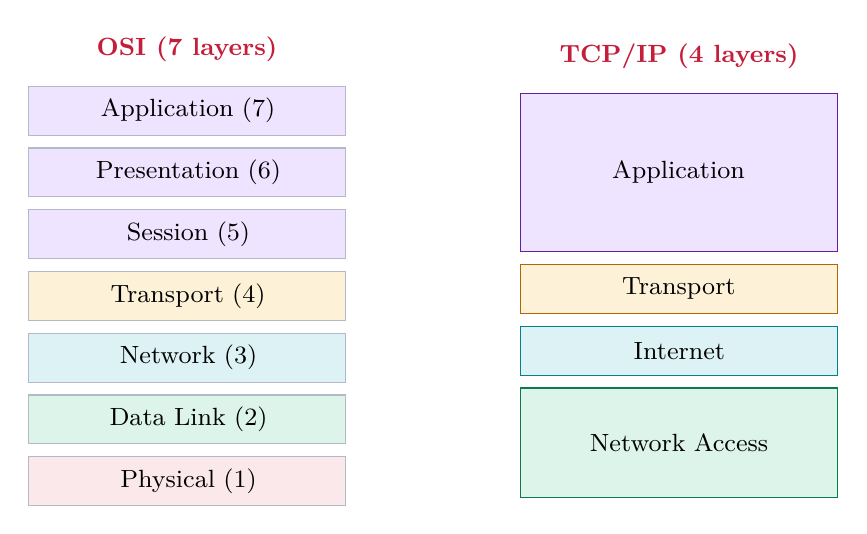
\begin{tikzpicture}[node distance=0.15cm]
  % OSI left column — 7 layers stacked top to bottom
  \node[rectangle, draw=mgframe, fill=hdrpurple, text width=3.8cm, align=center,
        minimum height=0.62cm, font=\small] (L7) {Application (7)};
  \node[rectangle, draw=mgframe, fill=hdrpurple, text width=3.8cm, align=center,
        minimum height=0.62cm, font=\small, below=0.15cm of L7] (L6) {Presentation (6)};
  \node[rectangle, draw=mgframe, fill=hdrpurple, text width=3.8cm, align=center,
        minimum height=0.62cm, font=\small, below=0.15cm of L6] (L5) {Session (5)};
  \node[rectangle, draw=mgframe, fill=hdramber, text width=3.8cm, align=center,
        minimum height=0.62cm, font=\small, below=0.15cm of L5] (L4) {Transport (4)};
  \node[rectangle, draw=mgframe, fill=hdrteal, text width=3.8cm, align=center,
        minimum height=0.62cm, font=\small, below=0.15cm of L4] (L3) {Network (3)};
  \node[rectangle, draw=mgframe, fill=hdrgreen, text width=3.8cm, align=center,
        minimum height=0.62cm, font=\small, below=0.15cm of L3] (L2) {Data Link (2)};
  \node[rectangle, draw=mgframe, fill=hdrred, text width=3.8cm, align=center,
        minimum height=0.62cm, font=\small, below=0.15cm of L2] (L1) {Physical (1)};
  % OSI label
  \node[above=0.18cm of L7, font=\small\bfseries\color{myred}] {OSI (7 layers)};
  % TCP/IP right column — 4 layers
  \node[rectangle, draw=mypurple, fill=hdrpurple, text width=3.8cm, align=center,
        minimum height=2.01cm, font=\small, right=2.2cm of L6] (app) {Application};
  \node[rectangle, draw=myamber, fill=hdramber, text width=3.8cm, align=center,
        minimum height=0.62cm, font=\small, below=0.15cm of app] (trans) {Transport};
  \node[rectangle, draw=myteal, fill=hdrteal, text width=3.8cm, align=center,
        minimum height=0.62cm, font=\small, below=0.15cm of trans] (inet) {Internet};
  \node[rectangle, draw=mygreen, fill=hdrgreen, text width=3.8cm, align=center,
        minimum height=1.39cm, font=\small, below=0.15cm of inet] (netacc) {Network Access};
  % TCP/IP label
  \node[above=0.18cm of app, font=\small\bfseries\color{myred}] {TCP/IP (4 layers)};
\end{tikzpicture}
\end{tcolorbox}

%═══════════════════════════════════════════════════════════════════════════════
\section{Physical Level}
%═══════════════════════════════════════════════════════════════════════════════

\subsection{Analog vs.\ Digital Data and Signals}

\begin{tabularx}{\linewidth}{|B{3.0cm}|X|X|}
\hline
\rowcolor{hdrgray}
\multicolumn{1}{|>{\centering\arraybackslash}p{3.0cm}|}{\textbf{Aspect}} &
\multicolumn{1}{>{\centering\arraybackslash}X|}{\textbf{\color{myteal}Analog}} &
\multicolumn{1}{>{\centering\arraybackslash}X|}{\textbf{\color{myamber}Digital}} \\
\hline
Data            & Continuous values (e.g.\ voice, temperature) & Discrete values (0 and 1) \\
\hline
\rowcolor{rowalt}
Signal          & Continuous waveform (sine wave) & Square wave / pulse train \\
\hline
Noise immunity  & Low --- noise degrades signal & High --- regenerated at repeaters \\
\hline
\rowcolor{rowalt}
Bandwidth       & Lower bandwidth needed & Higher bandwidth required \\
\hline
Transmission    & Analog transmission (amplifiers) & Digital transmission (repeaters) \\
\hline
\end{tabularx}

\subsection{Transmission Media}

\begin{tcolorbox}[defbox]
\textbf{Transmission Medium:} The physical path between sender and receiver. Classified as \textbf{guided} (wired) or \textbf{unguided} (wireless).
\end{tcolorbox}

\textbf{Guided Media:}
\begin{itemize}[leftmargin=*, itemsep=3pt]
  \item \textbf{Twisted Pair Cable:} Two insulated copper wires twisted together. Reduces electromagnetic interference. Types: UTP (Unshielded) and STP (Shielded). Used in telephone lines, Ethernet (Cat5e, Cat6).
  \item \textbf{Coaxial Cable:} Central conductor surrounded by insulation, metallic shield, and outer jacket. Higher bandwidth than twisted pair. Used in cable TV, older Ethernet (10Base2, 10Base5).
  \item \textbf{Fibre Optic Cable:} Transmits data as light pulses through glass/plastic core. Extremely high bandwidth, immune to EMI, low attenuation. Used in backbone networks, long-distance links.
\end{itemize}

\textbf{Unguided Media (Wireless):}
\begin{itemize}[leftmargin=*, itemsep=3pt]
  \item \textbf{Radio Waves:} Omnidirectional; penetrate walls. Used in AM/FM radio, Wi-Fi, Bluetooth.
  \item \textbf{Microwaves:} Directional; line-of-sight required. Used in satellite communication, cellular networks.
  \item \textbf{Infrared:} Short range; cannot penetrate walls. Used in TV remotes, IrDA.
\end{itemize}

\subsection{Circuit Switching}

\begin{tcolorbox}[defbox]
\textbf{Circuit Switching:} A dedicated communication path is established between sender and receiver for the entire duration of the session. Resources are reserved end-to-end. Used in traditional telephone networks (PSTN).
\end{tcolorbox}

\textbf{Phases of Circuit Switching:}
\begin{enumerate}[label=\textbf{\arabic*.}, leftmargin=*, itemsep=3pt]
  \item \textbf{Circuit Establishment:} A dedicated path is set up through intermediate switches.
  \item \textbf{Data Transfer:} Data flows continuously along the reserved path.
  \item \textbf{Circuit Disconnect:} Path is released and resources freed after communication ends.
\end{enumerate}

\subsubsection*{Space Division Switch}

\begin{tcolorbox}[formulabox, title={\textbf{Space Division Switching}}]
Each connection uses a \textbf{physically separate path} through the switch matrix. A crosspoint (transistor/relay) is activated at the intersection of input and output lines.\\[4pt]
\textbf{Crosspoint matrix:} For $n$ inputs and $n$ outputs, requires $n^2$ crosspoints.\\
\textbf{Advantage:} Simple, simultaneous connections. \textbf{Disadvantage:} Expensive for large $n$.
\end{tcolorbox}

\subsubsection*{Time Division Switch (TDM Bus)}

\begin{tcolorbox}[formulabox, title={\textbf{Time Division Switching}}]
All connections share the \textbf{same physical medium} but are separated in \textbf{time slots}. A Time Slot Interchange (TSI) unit reads input slots and writes them to output slots.\\[4pt]
\textbf{TDM Bus:} A high-speed shared bus; each input is assigned a time slot. The TSI reorders slots to route data to correct outputs.\\
\textbf{Advantage:} Efficient use of medium. \textbf{Disadvantage:} Requires synchronisation.
\end{tcolorbox}

\subsection{Telephone Network}

The Public Switched Telephone Network (PSTN) uses circuit switching. It consists of:
\begin{itemize}[leftmargin=*, itemsep=3pt]
  \item \textbf{Local loops:} Twisted pair from subscriber to local exchange (last mile).
  \item \textbf{Trunks:} High-capacity links (fibre/microwave) between exchanges.
  \item \textbf{Switching offices:} Local, tandem, and toll offices that route calls.
\end{itemize}

\begin{tcolorbox}[tikzbox, title={Telephone Network Structure}]
\centering
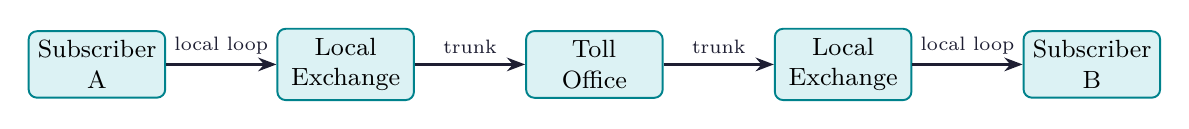
\begin{tikzpicture}[node distance=0.5cm and 1.4cm]
  \node[netnode] (sub1) {Subscriber\\A};
  \node[netnode, right=1.4cm of sub1] (local1) {Local\\Exchange};
  \node[netnode, right=1.4cm of local1] (toll) {Toll\\Office};
  \node[netnode, right=1.4cm of toll] (local2) {Local\\Exchange};
  \node[netnode, right=1.4cm of local2] (sub2) {Subscriber\\B};
  \draw[arrow] (sub1) -- node[above]{\scriptsize local loop} (local1);
  \draw[arrow] (local1) -- node[above]{\scriptsize trunk} (toll);
  \draw[arrow] (toll) -- node[above]{\scriptsize trunk} (local2);
  \draw[arrow] (local2) -- node[above]{\scriptsize local loop} (sub2);
\end{tikzpicture}
\end{tcolorbox}

%═══════════════════════════════════════════════════════════════════════════════
\section{Multiplexing: FDM, TDM, and WDM}
%═══════════════════════════════════════════════════════════════════════════════

\begin{tcolorbox}[defbox]
\textbf{Multiplexing:} A technique that allows multiple signals to share a single transmission medium simultaneously. A \textbf{multiplexer (MUX)} combines signals at the sender; a \textbf{demultiplexer (DEMUX)} separates them at the receiver.
\end{tcolorbox}

\begin{tcolorbox}[tikzbox, title={General Multiplexing Concept}]
\centering
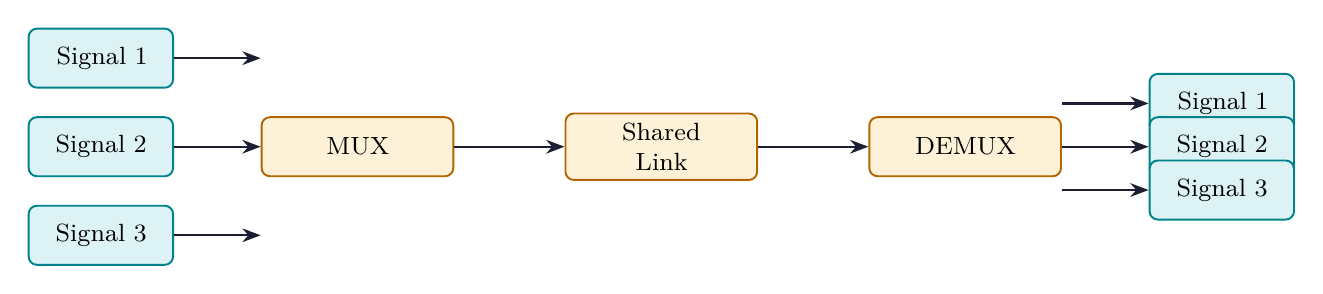
\begin{tikzpicture}[node distance=0.3cm and 0.9cm,
  sblock/.style={rectangle, draw=myteal, fill=hdrteal, text width=1.6cm,
    align=center, minimum height=0.75cm, font=\small, rounded corners=3pt, line width=0.7pt},
  chan/.style={rectangle, draw=myamber, fill=hdramber, text width=2.2cm,
    align=center, minimum height=0.75cm, font=\small, rounded corners=3pt, line width=0.7pt}]
  % Input signals
  \node[sblock] (s1) {Signal 1};
  \node[sblock, below=0.35cm of s1] (s2) {Signal 2};
  \node[sblock, below=0.35cm of s2] (s3) {Signal 3};
  % MUX
  \node[chan, right=1.1cm of s2] (mux) {MUX};
  % Shared link
  \node[chan, right=1.4cm of mux] (link) {Shared\\Link};
  % DEMUX
  \node[chan, right=1.4cm of link] (demux) {DEMUX};
  % Output signals
  \node[sblock, right=1.1cm of demux, yshift=0.55cm] (r1) {Signal 1};
  \node[sblock, right=1.1cm of demux] (r2) {Signal 2};
  \node[sblock, right=1.1cm of demux, yshift=-0.55cm] (r3) {Signal 3};
  % Arrows in
  \draw[arrow] (s1.east) -- (mux.west |- s1.east);
  \draw[arrow] (s2.east) -- (mux.west);
  \draw[arrow] (s3.east) -- (mux.west |- s3.east);
  % MUX to link to DEMUX
  \draw[arrow] (mux) -- (link);
  \draw[arrow] (link) -- (demux);
  % Arrows out
  \draw[arrow] (demux.east |- r1.west) -- (r1.west);
  \draw[arrow] (demux.east) -- (r2.west);
  \draw[arrow] (demux.east |- r3.west) -- (r3.west);
\end{tikzpicture}
\end{tcolorbox}

%───────────────────────────────────────────────────────────────────────────────
\subsection{Frequency Division Multiplexing (FDM)}
%───────────────────────────────────────────────────────────────────────────────

\begin{tcolorbox}[defbox]
\textbf{FDM (Frequency Division Multiplexing):} The total bandwidth of the medium is divided into non-overlapping \textbf{frequency bands (sub-channels)}. Each signal is modulated onto a different carrier frequency and transmitted simultaneously. Used for \textbf{analog signals}.
\end{tcolorbox}

\textbf{Working:}
\begin{enumerate}[label=\textbf{\arabic*.}, leftmargin=*, itemsep=3pt]
  \item Each input signal is modulated onto a unique carrier frequency $f_1, f_2, \ldots, f_n$.
  \item Guard bands (unused frequency gaps) separate adjacent channels to prevent interference.
  \item All modulated signals are combined and transmitted over the shared medium.
  \item At the receiver, bandpass filters separate each channel; demodulation recovers the original signal.
\end{enumerate}

\begin{tcolorbox}[formulabox, title={\textbf{FDM Key Formulas}}]
\begin{tabularx}{\linewidth}{B{4.5cm} X}
Channel bandwidth    & $B_{ch} = f_{upper} - f_{lower}$ \\[4pt]
Total bandwidth      & $B_{total} = n \times B_{ch} + (n-1) \times B_{guard}$ \\[4pt]
Guard band           & Unused frequency gap between adjacent channels to prevent inter-channel interference \\[4pt]
Carrier frequencies  & $f_1 < f_2 < \cdots < f_n$, each separated by at least $B_{ch} + B_{guard}$
\end{tabularx}
\end{tcolorbox}

\begin{tcolorbox}[tikzbox, title={FDM --- Frequency Spectrum Allocation}]
\centering
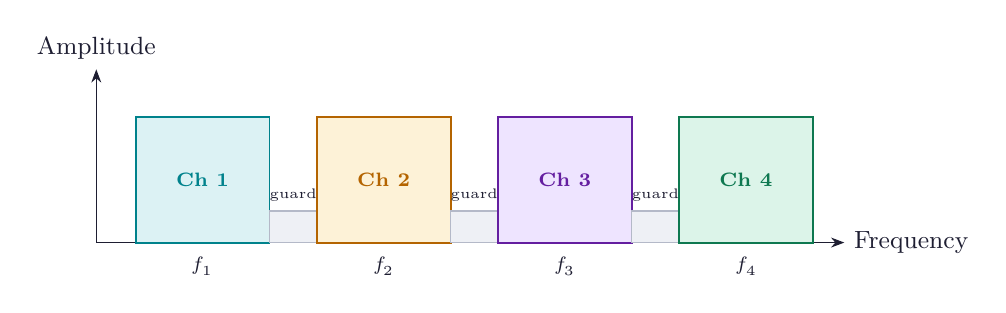
\begin{tikzpicture}[scale=1.0]
  % Frequency axis
  \draw[-Stealth, thin, color=mydark] (0,0) -- (9.5,0) node[right, font=\small] {Frequency};
  \draw[-Stealth, thin, color=mydark] (0,0) -- (0,2.2) node[above, font=\small] {Amplitude};
  % Channel 1
  \fill[hdrteal, draw=myteal, line width=0.7pt] (0.5,0) rectangle (2.2,1.6);
  \node[font=\scriptsize\bfseries, color=myteal] at (1.35,0.8) {Ch 1};
  \node[font=\scriptsize, color=mydark] at (1.35,-0.3) {$f_1$};
  % Guard band 1
  \fill[hdrgray, draw=mgframe, line width=0.5pt] (2.2,0) rectangle (2.8,0.4);
  \node[font=\tiny, color=mydark] at (2.5,0.6) {guard};
  % Channel 2
  \fill[hdramber, draw=myamber, line width=0.7pt] (2.8,0) rectangle (4.5,1.6);
  \node[font=\scriptsize\bfseries, color=myamber] at (3.65,0.8) {Ch 2};
  \node[font=\scriptsize, color=mydark] at (3.65,-0.3) {$f_2$};
  % Guard band 2
  \fill[hdrgray, draw=mgframe, line width=0.5pt] (4.5,0) rectangle (5.1,0.4);
  \node[font=\tiny, color=mydark] at (4.8,0.6) {guard};
  % Channel 3
  \fill[hdrpurple, draw=mypurple, line width=0.7pt] (5.1,0) rectangle (6.8,1.6);
  \node[font=\scriptsize\bfseries, color=mypurple] at (5.95,0.8) {Ch 3};
  \node[font=\scriptsize, color=mydark] at (5.95,-0.3) {$f_3$};
  % Guard band 3
  \fill[hdrgray, draw=mgframe, line width=0.5pt] (6.8,0) rectangle (7.4,0.4);
  \node[font=\tiny, color=mydark] at (7.1,0.6) {guard};
  % Channel 4
  \fill[hdrgreen, draw=mygreen, line width=0.7pt] (7.4,0) rectangle (9.1,1.6);
  \node[font=\scriptsize\bfseries, color=mygreen] at (8.25,0.8) {Ch 4};
  \node[font=\scriptsize, color=mydark] at (8.25,-0.3) {$f_4$};
\end{tikzpicture}
\end{tcolorbox}

\begin{tabularx}{\linewidth}{|B{3.2cm}|X|}
\hline
\rowcolor{hdrteal}
\multicolumn{1}{|>{\centering\arraybackslash}p{3.2cm}|}{\textbf{\color{myteal}Aspect}} &
\multicolumn{1}{>{\centering\arraybackslash}X|}{\textbf{\color{myteal}Details}} \\
\hline
Signal type       & Analog signals \\
\hline
\rowcolor{rowalt}
Separation method & Different carrier frequencies; guard bands prevent overlap \\
\hline
Simultaneous?     & Yes --- all channels transmit at the same time \\
\hline
\rowcolor{rowalt}
Applications      & AM/FM radio, cable TV, ADSL, first-generation cellular (1G) \\
\hline
Advantage         & Simple; no synchronisation needed; all channels always active \\
\hline
\rowcolor{rowalt}
Disadvantage      & Guard bands waste bandwidth; susceptible to intermodulation noise \\
\hline
\end{tabularx}

%───────────────────────────────────────────────────────────────────────────────
\subsection{Time Division Multiplexing (TDM)}
%───────────────────────────────────────────────────────────────────────────────

\begin{tcolorbox}[defbox]
\textbf{TDM (Time Division Multiplexing):} The time on the shared channel is divided into fixed \textbf{time slots}. Each input signal is assigned a slot in a repeating \textbf{frame}. Used for \textbf{digital signals}.
\end{tcolorbox}

\textbf{Two types of TDM:}

\begin{tcolorbox}[formulabox, title={\textbf{Synchronous TDM}}]
Each input is assigned a \textbf{fixed time slot} in every frame, regardless of whether it has data to send. Slots are pre-allocated.\\[4pt]
\begin{tabularx}{\linewidth}{B{4.0cm} X}
Frame duration    & $T_f = n \times T_s$ \quad ($n$ = number of channels, $T_s$ = slot duration) \\[4pt]
Output bit rate   & $R_{out} = n \times R_{in}$ \quad (output must be $n$ times faster than each input) \\[4pt]
Frame efficiency  & Can be low --- empty slots wasted if a channel has no data
\end{tabularx}
\end{tcolorbox}

\begin{tcolorbox}[formulabox, title={\textbf{Statistical (Asynchronous) TDM}}]
Slots are allocated \textbf{dynamically} --- only to channels that have data. Each slot carries an \textbf{address header} to identify the source.\\[4pt]
\begin{tabularx}{\linewidth}{B{4.0cm} X}
Efficiency        & Higher than synchronous TDM; no wasted slots \\[4pt]
Overhead          & Address field added to each slot increases overhead \\[4pt]
Output bit rate   & Less than $n \times R_{in}$ (statistical multiplexing gain)
\end{tabularx}
\end{tcolorbox}

\begin{tcolorbox}[tikzbox, title={Synchronous TDM --- Frame Structure (4 channels)}]
\centering
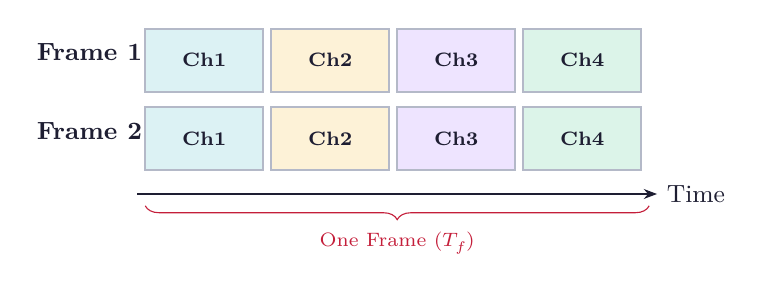
\begin{tikzpicture}[scale=1.0]
  % Frame label
  \node[font=\small\bfseries\color{mydark}, anchor=west] at (0, 1.6) {Frame 1:};
  % 4 slots in frame 1
  \foreach \i/\col/\lbl in {0/hdrteal/Ch1, 1/hdramber/Ch2, 2/hdrpurple/Ch3, 3/hdrgreen/Ch4} {
    \fill[\col, draw=mgframe, line width=0.7pt] ({1.5+\i*1.6}, 1.1) rectangle ({1.5+\i*1.6+1.5}, 1.9);
    \node[font=\scriptsize\bfseries\color{mydark}] at ({1.5+\i*1.6+0.75}, 1.5) {\lbl};
  }
  % Frame 2
  \node[font=\small\bfseries\color{mydark}, anchor=west] at (0, 0.6) {Frame 2:};
  \foreach \i/\col/\lbl in {0/hdrteal/Ch1, 1/hdramber/Ch2, 2/hdrpurple/Ch3, 3/hdrgreen/Ch4} {
    \fill[\col, draw=mgframe, line width=0.7pt] ({1.5+\i*1.6}, 0.1) rectangle ({1.5+\i*1.6+1.5}, 0.9);
    \node[font=\scriptsize\bfseries\color{mydark}] at ({1.5+\i*1.6+0.75}, 0.5) {\lbl};
  }
  % Time arrow
  \draw[-Stealth, thin, color=mydark] (1.4, -0.2) -- (8.0, -0.2) node[right, font=\small] {Time};
  % Brace for one frame
  \draw[decorate, decoration={brace, amplitude=5pt, mirror}, color=myred]
    (1.5, -0.35) -- (7.9, -0.35) node[midway, below=6pt, font=\scriptsize\color{myred}] {One Frame ($T_f$)};
\end{tikzpicture}
\end{tcolorbox}

\begin{tabularx}{\linewidth}{|B{3.2cm}|X|X|}
\hline
\rowcolor{hdrteal}
\multicolumn{1}{|>{\centering\arraybackslash}p{3.2cm}|}{\textbf{\color{myteal}Aspect}} &
\multicolumn{1}{>{\centering\arraybackslash}X|}{\textbf{\color{myteal}Synchronous TDM}} &
\multicolumn{1}{>{\centering\arraybackslash}X|}{\textbf{\color{myteal}Statistical TDM}} \\
\hline
Slot allocation   & Fixed; pre-assigned per channel & Dynamic; only active channels get slots \\
\hline
\rowcolor{rowalt}
Address header    & Not needed (position identifies channel) & Required (slot carries source address) \\
\hline
Efficiency        & Low if channels idle & High; no wasted slots \\
\hline
\rowcolor{rowalt}
Output rate       & $n \times R_{in}$ (fixed) & Less than $n \times R_{in}$ \\
\hline
Example           & T1/E1 lines, SONET & ATM, packet-switched networks \\
\hline
\end{tabularx}

%───────────────────────────────────────────────────────────────────────────────
\subsection{Wavelength Division Multiplexing (WDM)}
%───────────────────────────────────────────────────────────────────────────────

\begin{tcolorbox}[defbox]
\textbf{WDM (Wavelength Division Multiplexing):} Multiple optical signals are transmitted simultaneously over a single \textbf{fibre optic cable}, each on a different \textbf{wavelength (colour) of light}. Conceptually identical to FDM but applied to optical frequencies. Used in high-capacity fibre networks.
\end{tcolorbox}

\textbf{Working:}
\begin{enumerate}[label=\textbf{\arabic*.}, leftmargin=*, itemsep=3pt]
  \item Each data stream modulates a laser of a distinct wavelength $\lambda_1, \lambda_2, \ldots, \lambda_n$.
  \item A \textbf{prism or optical multiplexer} combines all wavelengths onto one fibre.
  \item The combined beam travels through the fibre.
  \item At the receiver, a \textbf{prism or optical demultiplexer} separates the wavelengths.
  \item Each wavelength is detected by a photodetector and demodulated.
\end{enumerate}

\begin{tcolorbox}[tikzbox, title={WDM --- Wavelength Multiplexing on Fibre}]
\centering
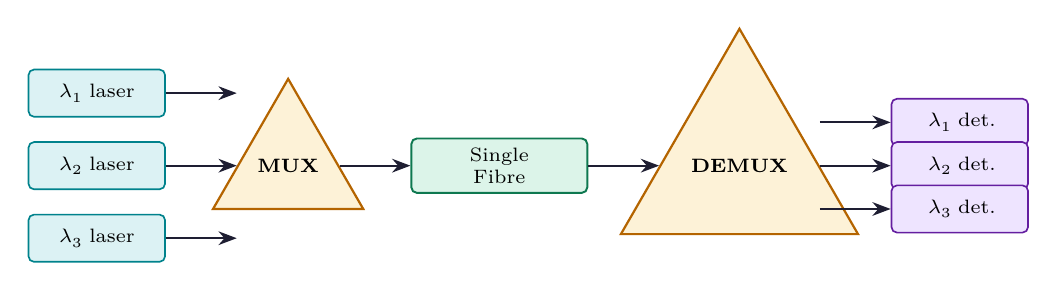
\begin{tikzpicture}[node distance=0.3cm and 0.8cm,
  laser/.style={rectangle, draw=myteal, fill=hdrteal, text width=1.5cm,
    align=center, minimum height=0.6cm, font=\scriptsize, rounded corners=2pt, line width=0.6pt},
  prism/.style={regular polygon, regular polygon sides=3, draw=myamber, fill=hdramber,
    minimum size=1.1cm, font=\scriptsize\bfseries, inner sep=0pt, line width=0.8pt},
  fibre/.style={rectangle, draw=mygreen, fill=hdrgreen, text width=2.0cm,
    align=center, minimum height=0.6cm, font=\scriptsize, rounded corners=2pt, line width=0.7pt},
  det/.style={rectangle, draw=mypurple, fill=hdrpurple, text width=1.5cm,
    align=center, minimum height=0.6cm, font=\scriptsize, rounded corners=2pt, line width=0.6pt}]
  % Lasers
  \node[laser] (l1) {$\lambda_1$ laser};
  \node[laser, below=0.3cm of l1] (l2) {$\lambda_2$ laser};
  \node[laser, below=0.3cm of l2] (l3) {$\lambda_3$ laser};
  % MUX prism
  \node[prism, right=0.9cm of l2] (mux) {MUX};
  % Fibre
  \node[fibre, right=0.9cm of mux] (fibre) {Single\\Fibre};
  % DEMUX prism
  \node[prism, right=0.9cm of fibre] (demux) {DEMUX};
  % Detectors
  \node[det, right=0.9cm of demux, yshift=0.55cm] (d1) {$\lambda_1$ det.};
  \node[det, right=0.9cm of demux] (d2) {$\lambda_2$ det.};
  \node[det, right=0.9cm of demux, yshift=-0.55cm] (d3) {$\lambda_3$ det.};
  % Arrows
  \draw[arrow] (l1.east) -- (mux.west |- l1.east);
  \draw[arrow] (l2.east) -- (mux.west);
  \draw[arrow] (l3.east) -- (mux.west |- l3.east);
  \draw[arrow] (mux.east) -- (fibre.west);
  \draw[arrow] (fibre.east) -- (demux.west);
  \draw[arrow] (demux.east |- d1.west) -- (d1.west);
  \draw[arrow] (demux.east) -- (d2.west);
  \draw[arrow] (demux.east |- d3.west) -- (d3.west);
\end{tikzpicture}
\end{tcolorbox}

\textbf{Types of WDM:}
\begin{itemize}[leftmargin=*, itemsep=3pt]
  \item \textbf{CWDM (Coarse WDM):} Fewer channels (up to 18), wider wavelength spacing (20 nm). Lower cost, shorter distances.
  \item \textbf{DWDM (Dense WDM):} Many channels (40--160+), very narrow spacing (0.8 nm or less). Used in long-haul backbone networks. Capacity up to several Tbps on one fibre.
\end{itemize}

\begin{tabularx}{\linewidth}{|B{3.2cm}|X|}
\hline
\rowcolor{hdrteal}
\multicolumn{1}{|>{\centering\arraybackslash}p{3.2cm}|}{\textbf{\color{myteal}Aspect}} &
\multicolumn{1}{>{\centering\arraybackslash}X|}{\textbf{\color{myteal}Details}} \\
\hline
Medium            & Fibre optic cable only \\
\hline
\rowcolor{rowalt}
Separation method & Different wavelengths (colours) of light \\
\hline
Analogy           & FDM applied to optical domain \\
\hline
\rowcolor{rowalt}
Capacity          & DWDM: 40--160+ channels; Tbps aggregate \\
\hline
Applications      & Internet backbone, long-haul telecom, submarine cables \\
\hline
\rowcolor{rowalt}
Advantage         & Enormous capacity; each wavelength is independent \\
\hline
Disadvantage      & Expensive equipment; requires precise laser wavelengths \\
\hline
\end{tabularx}

%───────────────────────────────────────────────────────────────────────────────
\subsection{FDM vs.\ TDM vs.\ WDM --- Comparison}
%───────────────────────────────────────────────────────────────────────────────

\par\noindent
\begin{tabularx}{\linewidth}{|B{3.0cm}|>{\small\raggedright\arraybackslash}X|>{\small\raggedright\arraybackslash}X|>{\small\raggedright\arraybackslash}X|}
\hline
\rowcolor{hdrgray}
\multicolumn{1}{|>{\centering\arraybackslash}p{3.0cm}|}{\textbf{Parameter}} &
\multicolumn{1}{>{\centering\arraybackslash}X|}{\textbf{\color{myteal}FDM}} &
\multicolumn{1}{>{\centering\arraybackslash}X|}{\textbf{\color{myamber}TDM}} &
\multicolumn{1}{>{\centering\arraybackslash}X|}{\textbf{\color{mygreen}WDM}} \\
\hline
Full form         & Frequency Division Multiplexing & Time Division Multiplexing & Wavelength Division Multiplexing \\
\hline
\rowcolor{rowalt}
Signal type       & Analog & Digital & Optical (light) \\
\hline
Sharing basis     & Frequency bands & Time slots & Wavelengths of light \\
\hline
\rowcolor{rowalt}
Medium            & Coaxial, twisted pair, air & Any digital medium & Fibre optic only \\
\hline
Synchronisation   & Not required & Required (sync TDM) & Not required \\
\hline
\rowcolor{rowalt}
Guard bands       & Required & Not needed & Not needed (wavelength spacing) \\
\hline
Applications      & Radio, cable TV, ADSL & T1/E1, SONET, GSM & Internet backbone, DWDM \\
\hline
\rowcolor{rowalt}
Capacity          & Moderate & High & Very high (Tbps) \\
\hline
\end{tabularx}

%═══════════════════════════════════════════════════════════════════════════════
% QUICK REVISION PAGE
%═══════════════════════════════════════════════════════════════════════════════
\newpage
\begin{center}
  {\large\bfseries\color{myred} Quick Revision --- Module 1}\\[3pt]
  {\small\color{mydark} Data Communication, Networking Overview \& Physical Level $|$ EC602}
\end{center}
\noindent{\color{myred}\rule{\linewidth}{1.2pt}}
\vspace{4pt}

\begin{tcolorbox}[formulabox, title={\textbf{Key Facts at a Glance}}]
\begin{tabularx}{\linewidth}{B{4.8cm} X}
OSI Layers (top to bottom) & Application, Presentation, Session, Transport, Network, Data Link, Physical \\[2pt]
TCP/IP Layers              & Application, Transport, Internet, Network Access \\[2pt]
LAN coverage               & Up to a few km (building/campus) \\[2pt]
MAN coverage               & City-wide (5--50 km) \\[2pt]
WAN coverage               & Country / global \\[2pt]
Simplex                    & One direction only \\[2pt]
Half Duplex                & Both directions, not simultaneously \\[2pt]
Full Duplex                & Both directions simultaneously \\[2pt]
Circuit switching phases   & Establish $\to$ Transfer $\to$ Disconnect \\[2pt]
Space division crosspoints & $n^2$ for $n \times n$ \\[2pt]
TDM output bit rate        & $R_{out} = n \times R_{in}$ (synchronous TDM) \\[2pt]
TDM frame duration         & $T_f = n \times T_s$ \\[2pt]
FDM total bandwidth        & $B_{total} = n \times B_{ch} + (n-1) \times B_{guard}$ \\[2pt]
WDM                        & FDM applied to optical domain; uses wavelengths of light switch \\[2pt]
ASCII                      & 7-bit encoding, 128 characters \\[2pt]
Unicode                    & 32-bit encoding, universal character set \\[2pt]
\end{tabularx}
\end{tcolorbox}

\vspace{6pt}

\begin{tcolorbox}[defbox, title={\textbf{One-Line Definitions}}]
\begin{itemize}[leftmargin=*, itemsep=3pt, topsep=0pt]
  \item \textbf{Protocol:} Set of rules governing communication between devices.
  \item \textbf{Topology:} Geometric arrangement of devices and links in a network.
  \item \textbf{LAN:} Local Area Network; high-speed network within a building or campus.
  \item \textbf{WAN:} Wide Area Network; spans cities, countries, or the globe.
  \item \textbf{OSI Model:} 7-layer ISO standard for network communication.
  \item \textbf{TCP/IP Model:} 4-layer practical model underlying the Internet.
  \item \textbf{Circuit Switching:} Dedicated path reserved for entire session duration.
  \item \textbf{TDM:} Time Division Multiplexing; shares medium by assigning time slots to each channel.
  \item \textbf{FDM:} Frequency Division Multiplexing; divides bandwidth into frequency bands for analog signals.
  \item \textbf{WDM:} Wavelength Division Multiplexing; uses different light wavelengths on a single fibre optic cable.
  \item \textbf{Statistical TDM:} Dynamic slot allocation; only active channels get slots, improving efficiency.
  \item \textbf{DWDM:} Dense WDM; 40--160+ channels with narrow wavelength spacing; used in backbone networks.
  \item \textbf{Guided Media:} Physical wired medium (twisted pair, coaxial, fibre optic).
  \item \textbf{Unguided Media:} Wireless medium (radio, microwave, infrared).
  \item \textbf{Full Duplex:} Simultaneous two-way communication.
  \item \textbf{ASCII:} American Standard Code for Information Interchange; 7-bit text encoding.
\end{itemize}
\end{tcolorbox}

\vspace{6pt}

\begin{tcolorbox}[exambox, title={\textbf{Frequently Asked / Viva Questions}}]
\begin{enumerate}[leftmargin=*, topsep=0pt, label=\textbf{Q\arabic*.}, itemsep=8pt]
  \item \Q{What are the five components of data communication?} Sender, Receiver, Message, Medium, and Protocol.
  \item \Q{Difference between simplex, half duplex, and full duplex?} Simplex: one direction only. Half duplex: both directions but not simultaneously. Full duplex: both directions simultaneously.
  \item \Q{How many layers does the OSI model have? Name them.} 7 layers: Physical, Data Link, Network, Transport, Session, Presentation, Application (bottom to top).
  \item \Q{What is the PDU at the Network layer?} Packet.
  \item \Q{What is the PDU at the Data Link layer?} Frame.
  \item \Q{How does TCP/IP differ from OSI?} TCP/IP has 4 layers vs.\ OSI's 7; TCP/IP is practical and protocol-specific; OSI is a conceptual reference model.
  \item \Q{What is circuit switching?} A dedicated communication path is established and reserved for the entire session. Used in PSTN.
  \item \Q{What is the difference between space division and time division switching?} Space division uses separate physical paths (crosspoint matrix); time division shares one medium using time slots (TSI).
  \item \Q{What is the advantage of fibre optic over copper?} Higher bandwidth, lower attenuation, immune to EMI, more secure.
  \item \Q{What is a MAN?} Metropolitan Area Network; covers a city (5--50 km); e.g.\ cable TV network, WiMAX.
  \item \Q{What does ASCII stand for?} American Standard Code for Information Interchange; 7-bit encoding for 128 characters.
  \item \Q{Why is full duplex preferred over half duplex?} Full duplex allows simultaneous two-way communication, doubling effective throughput compared to half duplex.
  \item \Q{What is multiplexing and why is it used?} Multiplexing allows multiple signals to share a single transmission medium, reducing cost and making efficient use of bandwidth.
  \item \Q{What is the difference between FDM and TDM?} FDM divides the bandwidth into frequency bands for analog signals; TDM divides time into slots for digital signals. FDM channels transmit simultaneously; TDM channels take turns.
  \item \Q{What is WDM and where is it used?} WDM transmits multiple optical signals on one fibre using different wavelengths of light. Used in Internet backbone and long-haul telecom (DWDM supports 40--160+ channels).
  \item \Q{What is the difference between synchronous and statistical TDM?} Synchronous TDM assigns fixed slots to each channel regardless of activity (wastes slots if idle). Statistical TDM allocates slots dynamically only to active channels, improving efficiency but requiring address headers.
\end{enumerate}
\end{tcolorbox}

\vspace{6pt}

\begin{tcolorbox}[tikzbox, title={\textbf{OSI Layer Summary Table}}]
\begin{tabularx}{\linewidth}{|>{\centering\arraybackslash}p{0.5cm}|B{2.8cm}|X|>{\centering\arraybackslash}p{2.2cm}|}
\hline
\rowcolor{hdrgray}
\textbf{\#} & \textbf{Layer} & \textbf{Key Function} & \textbf{PDU} \\
\hline
7 & Application  & User-facing services (HTTP, FTP, DNS) & Data \\
\hline
\rowcolor{rowalt}
6 & Presentation & Encryption, compression, translation & Data \\
\hline
5 & Session      & Session management, synchronisation & Data \\
\hline
\rowcolor{rowalt}
4 & Transport    & End-to-end delivery, TCP/UDP & Segment \\
\hline
3 & Network      & Routing, IP addressing & Packet \\
\hline
\rowcolor{rowalt}
2 & Data Link    & Framing, MAC, error detection & Frame \\
\hline
1 & Physical     & Bit transmission over medium & Bits \\
\hline
\end{tabularx}
\end{tcolorbox}

\end{document}
